\tikzset{>=latex} % for LaTeX arrow head
\contourlength{1.4pt}

\colorlet{Ecol}{orange!90!black}
\colorlet{EcolFL}{orange!90!black}
\colorlet{veccol}{green!45!black}
\colorlet{EFcol}{red!60!black}
\tikzstyle{charged}=[top color=blue!20,bottom color=blue!40,shading angle=10]
\tikzstyle{darkcharged}=[very thin,top color=blue!60,bottom color=blue!80,shading angle=10]
\tikzstyle{charge+}=[very thin,top color=red!80,bottom color=red!80!black,shading angle=-5]
\tikzstyle{charge-}=[very thin,top color=blue!50,bottom color=blue!70!white!90!black,shading angle=10]
\tikzstyle{darkcharged}=[very thin,top color=blue!60,bottom color=blue!80,shading angle=10]
\tikzstyle{gauss surf}=[green!70!black,top color=green!2,bottom color=green!80!black!70,shading angle=5,fill opacity=0.6]
\tikzstyle{gauss lid}=[gauss surf,middle color=green!80!black!20,shading angle=40,fill opacity=0.7]
\tikzstyle{gauss dark}=[green!60!black,fill=green!60!black!70,fill opacity=0.8]
\tikzstyle{gauss line}=[green!80!black]
\tikzstyle{gauss dashed line}=[green!60!black!80,dashed,line width=0.2]
\tikzstyle{vector}=[->,thick,veccol]
\tikzstyle{normalvec}=[->,thick,blue!80!black!80]
\tikzstyle{EField}=[->,thick,Ecol]
\tikzstyle{EField dashed}=[dashed,Ecol,line width=0.6]
\tikzset{
  EFieldLine/.style={thick,EcolFL,decoration={markings,
                     mark=at position #1 with {\arrow{latex}}},
                     postaction={decorate}},
  EFieldLine/.default=0.5}
\tikzstyle{measure}=[fill=white,midway,outer sep=2]
\def\L{2.2}
\def\H{2.2}
\def\offset{2.0}
\def\W{0.30}
\def\Nx{5}
\def\Ny{5}

% PLANE charge distribution




% ROUND SHEET integration


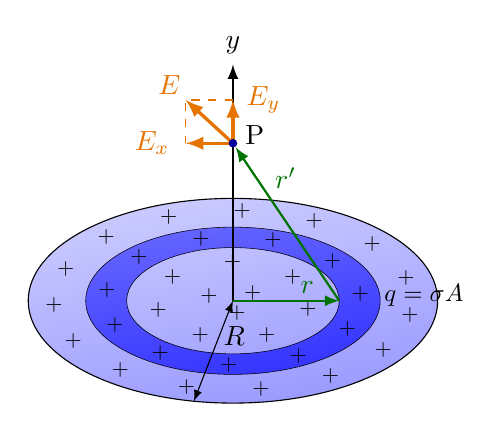
\begin{tikzpicture}[x={(1,0)},y={(0,0.5)}]
  \def\R{2.6}
  \def\r{1.35}
  \def\dr{0.52}
  \def\Ex{0.6}
  \def\Ey{1.1}
  \def\Nx{4}
  \coordinate (O) at (0,0);
  \coordinate (P) at (0,4.0);
  \coordinate (Y) at (0,6.0);
  \coordinate (R) at (\r,0);
  
  % PLANE
  \draw[charged]
    (O) circle (\R);
  \draw[darkcharged,even odd rule]
    (O) circle (\r+\dr) circle (\r);
  \foreach \i [evaluate={\cr=(\i-0.5)*\R/\Nx; \Ny=7+4*(\i-2);}] in {1,...,\Nx}{
    \foreach \j [evaluate={\cang=39+\j*360/\Ny;}] in {1,...,\Ny}{
      \node[scale=0.8,rotate=0] at (\cang:\cr) {$+$};
    }
  }
  
  % CHARGE
  \node[right=-1.5,scale=0.9] at (4:\r+\dr) {$\dd{q}=\sigma \dd{A}$};
  
  % AXIS
  \draw[->,thick] (0,0) -- (Y) node[above] {$y$};
  
  % VECTORS
  \draw[EField,very thick] (P) --++ ( 0.0,\Ey) node[right=1] {$\dd{\vb{E}_y}$};
  \draw[EField,very thick] (P) --++ (-\Ex,0.0) node[left=2] {$\dd{\vb{E}_x}$};
  \draw[EField,very thick] (P) --++ (-\Ex,\Ey) node[above left=-2] {$\dd{\vb{E}}$};
  \draw[EField,-,dashed,thin] (P) ++ (0,\Ey) --++ (-\Ex,0) --++ (0,-\Ey);
  \node[fill=blue!60!black,circle,inner sep=1.1] (P') at (P) { };
  \node[above=3,right=1] at (P') {P};
  \draw[vector,veccol] (R) -- (P') node[pos=0.8,right=3] {$\vb{r}'$};
  \draw[vector,veccol] (0,0) --++ (0:\r) node[pos=0.7,above=-1] {$\vb{r}$};
  \draw[<->] (0,0) --++ (-101:\R) node[pos=0.35,right=-2] {$R$};
  
\end{tikzpicture}
